\input{preambule_damien2.tex}     

%%%%%%%%%%%%%%%%%%%%%%%%%%%%%%%%%%%%%%%%%%%
%****************TABLEAUX*******************************%
%%%%%%%%%%%%%%%%%%%%%%%%%%%%%%%%%%%%%%%%%%%

%%%%%%%%%%%%%%%% TABLEAU SIGNE ET VARIATION %%%%%%%%%%%%%%
%\begin{center}
%%\vspace{0.3cm}
%\begin{tikzpicture}
%\tkzTabInit[espcl=2]{$x$ /.8 , $d(x)$ /1.5}{$0$ , $4$,$16$,$24$}
%\tkzTabLine[]{,+,z,-,}
%\tkzTabVar[]{+/ $8$,-/$6$,+/$19$,-/$8$}
%%\tkzTabVal[draw]{1}{2}{0.5}{0}{0}
%\end{tikzpicture}
%\end{center}

%%%%%%%%%%%%%%% TABLEAU %%%%%%%%%%%%%%%%%%%%%%%%%%%%%%
%\renewcommand{\arraystretch}{hauteur}
%\begin{center}
%\begin{tabularx}{0.94\linewidth}{|c|*{7}{>{\centering \arraybackslash}X|}}
%\hline 
%
%\hline 
%\end{tabularx} 
%\end{center}

%%%%%%%%%%%%%%%%%%%%%%%%%%%%%%%%%%%%%%%%%%%
%****************** GRAPHIQUE FCT**********************%
%%%%%%%%%%%%%%%%%%%%%%%%%%%%%%%%%%%%%%%%%%%

%\psset{xunit=0.75cm,yunit=0.75cm,algebraic=true,dimen=middle,dotstyle=o,dotsize=5pt 0,linewidth=1.4pt,arrowsize=2pt 2,arrowinset=0.25}
%\def\xmin{-9} \def\xmax{9} \def\ymin{-10.5} \def\ymax{6.5} \def\dx{0.5} \def\dy{0.5}
%\begin{center}
%		\begin{pspicture*}(\xmin,\ymin)(\xmax,\ymax)
%		\multips(0,\ymin)(0,\dy){35}{\psline[linestyle=dashed,linecap=1,dash=1.5pt 1.5pt,linewidth=0.4pt,linecolor=lightgray]{c-c}(\xmin,0)(\xmax,0)}
%		\multips(\xmin,0)(\dx,0){38}{\psline[linestyle=dashed,linecap=1,dash=1.5pt 1.5pt,linewidth=0.4pt,linecolor=lightgray]{c-c}(0,\ymin)(0,\ymax)}
%		\psaxes[labels=all,labelFontSize=\scriptstyle,labelsep=2pt,xAxis=true,yAxis=true,Dx=1,Dy=1,ticksize=-2pt 0,subticks=2,showorigin=False]{->}(0,0)(\xmin,\ymin)(\xmax,\ymax)[{$x$,0][$y$,90]
%\psclip{%
%\psframe[linestyle=none](\xmin,\ymin)(\xmax,\ymax)}
%		\uput[dl](0,0){\scriptsize $0$}
%		\psplot[linewidth=1.4pt,plotpoints=200, linecolor=blue]{\xmin}{\xmax}{2.79^x}
%}\endpsclip
%		\end{pspicture*}
%\end{center}

%%%%%%%%%%%%%%%%%%%%%%%%%%%%%%%%%%%%%%%%%%%
% *******************MINTED *****************************%
%%%%%%%%%%%%%%%%%%%%%%%%%%%%%%%%%%%%%%%%%%%
%\usepackage{minted}
%
%\renewcommand{\theFancyVerbLine}{\textcolor{gray}{\tiny \oldstylenums{\arabic{FancyVerbLine}}}}
%
%\definecolor{bg}{rgb}{0.95,0.95,0.95}
%
%\newminted[python]{python}{fontfamily=tt,linenos=true,autogobble,mathescape=true,python3,fontsize=\small, tabsize=4, samepage=true, rulecolor=gray, numbersep=2pt, bgcolor=bg}
%
%\newmintinline{python}{fontfamily=tt,linenos=true,autogobble,mathescape=true,python3}
%
%\newmintedfile[pythonexternal]{python}{fontfamily=tt,linenos=true,autogobble,mathescape=true,python3}
%
%\newminted[html]{html}{fontfamily=courier, fontsize=\footnotesize, rulecolor=gray, framerule=1.5pt, mathescape=true, texcomments=true, autogobble, tabsize=4, numbersep=8pt}
%
%\newmintinline{html}{fontfamily=courier, fontsize=\small}
%
%\newminted[css]{css}{fontfamily=courier, fontsize=\footnotesize, rulecolor=gray, framerule=1.5pt, mathescape=true, texcomments=true, autogobble, tabsize=4, numbersep=8pt}
%
%\newmintinline{css}{fontfamily=courier, fontsize=\small}
%
%\newminted[algo]{bbcode}{fontfamily=courier, fontsize=\footnotesize, rulecolor=gray, framerule=1.5pt, mathescape=true, texcomments=true, autogobble, linenos=true, tabsize=4, numbersep=8pt}

%%%%%%%%%%%%%%%%%%%%%%%%%%%%%%%%%%%%%%%%%%%
% *******************EnT�tes et Pieds de page *****************************%
%%%%%%%%%%%%%%%%%%%%%%%%%%%%%%%%%%%%%%%%%%%
\pagestyle{fancy}
\setlength{\headheight}{40pt} % Haut de page
\renewcommand{\headrulewidth}{0.0pt}
\setlength{\textheight}{26cm}
\lhead{}
%\chead{\thepage/\pageref{LastPage}}
\rhead{}
\renewcommand{\footrulewidth}{1pt}
\lfoot{2GT --- SNT}
\cfoot{}
%\rfoot{\thepage/\pageref{LastPage}}


%%%%%%%%%%%%%%%%%%%%%%%%%%%%%%%%%%%%%%%%%%%%%%

\usepackage{mdframed}

\begin{document}

\begin{titre}{2NDE}{Seconde - SNT}
\centering
{\Large \textsc{\textbf{Th�me : Internet --- S�ance 2}}}
\end{titre}

\newcommand{\tableroutage}[7]{
  \begin{tabular}{|c@{$\rightarrow$}c|}
    \multicolumn{2}{c}{\textbf{\large #1}} \\
    \hline
    A & #2 \\
    B & #3 \\
    C & #4 \\
    D & #5 \\
    E & #6 \\
    F & #7 \\
    \hline
  \end{tabular}
}

\section{R�seau fixe}

Dans le r�seau suivant, chaque routeur dispose d'une \emph{table de routage} pour transmettre un message : $A \rightarrow C$ signifie : \og Si j'ai un message � envoyer � $A$, je transmets ce message � $C$. \fg{}.

\begin{center}
  \footnotesize
  \begin{tikzpicture}[scale=1,very thick, xscale=1.8, yscale=1.2]
  \node (A) at (0, 4) {\tableroutage{A}{ }{C}{C}{C}{C}{C}};
  \node (B) at (4, 4) {\tableroutage{B}{C}{ }{C}{D}{C}{D}};
  \node (C) at (2, 2) {\tableroutage{C}{A}{B}{ }{B}{E}{F}};
  \node (D) at (6, 2) {\tableroutage{D}{F}{B}{B}{ }{F}{F}};
  \node (E) at (0, 0) {\tableroutage{E}{A}{F}{C}{C}{ }{F}};
  \node (F) at (4, 0) {\tableroutage{F}{E}{D}{C}{D}{E}{ }};
  \draw (A) -- (C) -- (B) -- (D) -- (F) -- (C) -- (E) -- (F);
  \end{tikzpicture}
\end{center}

\begin{enumerate}
  \item Le routeur $E$ doit transmettre un message � $D$. En utilisant exclusivement les tables de routage, par quel chemin va passer le message ?
	\vspace*{1.6cm}
  \item Le routeur $D$ r�pond � $E$. Avec la m�me contrainte, par quel chemin va passer la r�ponse ?
	\vspace*{1.6cm}
	
	\item Le routeur $F$ veut transmettre � $A$ : rep�rez et corrigez l'erreur \dots
	
	\vspace*{1.6cm}
	
\end{enumerate}

\section{R�seau mouvant}

La connexion entre les routeurs $E$ et $F$ est perdue. Sachant que chaque routeur ne peut dialoguer qu'avec les routeurs auxquels il est directement connect�, comment est-il possible de mettre � jour l'ensemble des tables de routage, pour que $D$ puisse � nouveau envoyer un message � $E$ ?

\end{document}
